\documentclass{article}
\usepackage{amsmath}
\usepackage{graphicx}
\usepackage{geometry}
\usepackage{booktabs}
\usepackage[hidelinks]{hyperref}
\usepackage{xcolor}
\usepackage{mdframed}
\usepackage{enumitem}
\usepackage{longtable}
\usepackage{multirow}
\usepackage{gensymb}
\usepackage{float}
\usepackage{placeins}
\usepackage{caption}
\usepackage{array}

\geometry{margin=1.5cm}
\setlength{\parindent}{0pt}
\setlength{\parskip}{0.35em}
\setlength{\tabcolsep}{6pt}
\renewcommand{\arraystretch}{1.12}
\captionsetup{font=small, labelfont=bf}

\title{\textbf{ Data to Design} \\ \large Linear Model Family Report}
\author{S1 Linear Family}
\date{July 2026}

\begin{document}
\maketitle
\tableofcontents
\clearpage

% ============================================================
\section{Results and Interpretation}
% ============================================================

\subsection{IID Baseline Results}
This subsection presents the baseline performance of the Linear Model Family on the UCI Concrete dataset and the UHPC dataset. The tested models were Ordinary Least Squares (OLS), Elastic Net, Bayesian Ridge, and Polynomial Ridge.

\subsubsection{UCI Dataset}

The UCI experiments used an 80/20 train-test split. Hyperparameter tuning was performed with 4-fold cross-validation, following the four-part validation idea used in Yeh's original concrete strength study.

\begin{table}[H]
\centering

\begin{minipage}[t]{0.48\textwidth}
\centering
\textbf{Original Dataset}\\[0.4em]
\begin{tabular}{@{}lllll@{}}
\toprule
\textbf{Model} & \textbf{MAE} & \textbf{RMSE} & \textbf{R} & \textbf{$R^2$} \\
\midrule
OLS              & 8.72 & 10.94 & 0.790 & 0.617 \\
Elastic Net      & 8.75 & 10.95 & 0.790 & 0.616 \\
Bayesian Ridge   & 8.75 & 10.95 & 0.790 & 0.616 \\
Polynomial Ridge & 4.69 &  6.57 & 0.929 & 0.862 \\
\bottomrule
\end{tabular}
\end{minipage}
\hfill
\begin{minipage}[t]{0.48\textwidth}
\centering
\textbf{Domain-Ratio Dataset}\\[0.4em]
\begin{tabular}{@{}lllll@{}}
\toprule
\textbf{Model} & \textbf{MAE} & \textbf{RMSE} & \textbf{R} & \textbf{$R^2$} \\
\midrule
OLS              & 8.45 & 10.69 & 0.803 & 0.634 \\
Elastic Net      & 8.58 & 10.76 & 0.803 & 0.629 \\
Bayesian Ridge   & 8.49 & 10.71 & 0.803 & 0.633 \\
Polynomial Ridge & 4.72 &  6.71 & 0.926 & 0.856 \\
\bottomrule
\end{tabular}
\end{minipage}

\vspace{1em}

\begin{minipage}[t]{0.48\textwidth}
\centering
\textbf{Log-Transformed Dataset}\\[0.4em]
\begin{tabular}{@{}lllll@{}}
\toprule
\textbf{Model} & \textbf{MAE} & \textbf{RMSE} & \textbf{R} & \textbf{$R^2$} \\
\midrule
OLS              & 4.88 & 6.48 & 0.931 & 0.865 \\
Elastic Net      & 4.87 & 6.48 & 0.932 & 0.866 \\
Bayesian Ridge   & 4.86 & 6.48 & 0.932 & 0.866 \\
Polynomial Ridge & 4.03 & 5.80 & 0.946 & 0.892 \\
\bottomrule
\end{tabular}
\end{minipage}
\hfill
\begin{minipage}[t]{0.48\textwidth}
\centering
\textbf{Interaction Dataset}\\[0.4em]
\begin{tabular}{@{}lllll@{}}
\toprule
\textbf{Model} & \textbf{MAE} & \textbf{RMSE} & \textbf{R} & \textbf{$R^2$} \\
\midrule
OLS              & 4.49 & 6.19 & 0.938 & 0.877 \\
Elastic Net      & 4.47 & 6.18 & 0.939 & 0.878 \\
Bayesian Ridge   & 4.48 & 6.18 & 0.939 & 0.878 \\
Polynomial Ridge & 3.78 & 5.66 & 0.949 & 0.897 \\
\bottomrule
\end{tabular}
\end{minipage}

\caption{Linear-family baseline and feature-representation results on the UCI Concrete dataset.}
\end{table}

\paragraph{Summary}
\begin{center}
\begin{tabular}{@{}llll@{}}
\toprule
\textbf{Dataset} & \textbf{Best Model} & \textbf{RMSE} & \textbf{$R^2$} \\
\midrule
Original Dataset        & Polynomial Ridge & 6.57 & 0.862 \\
Domain-Ratio Dataset    & Polynomial Ridge & 6.71 & 0.856 \\
Log-Transformed Dataset & Polynomial Ridge & 5.80 & 0.892 \\
Interaction Dataset     & Polynomial Ridge & 5.66 & 0.897 \\
\bottomrule
\end{tabular}
\end{center}

\paragraph{Interpretation}
The plain linear models were too simple for the UCI dataset, staying near RMSE 10.9 and $R^2 \approx 0.62$ on the original variables. Polynomial Ridge performed much better because it can represent curved effects such as age gain and nonlinear mix-ratio behavior. The interaction dataset was the strongest setup, and across three random seeds the Polynomial Ridge model achieved RMSE $5.17 \pm 0.49$ and $R^2 = 0.901 \pm 0.007$.

\begin{figure}[H]
    \centering
    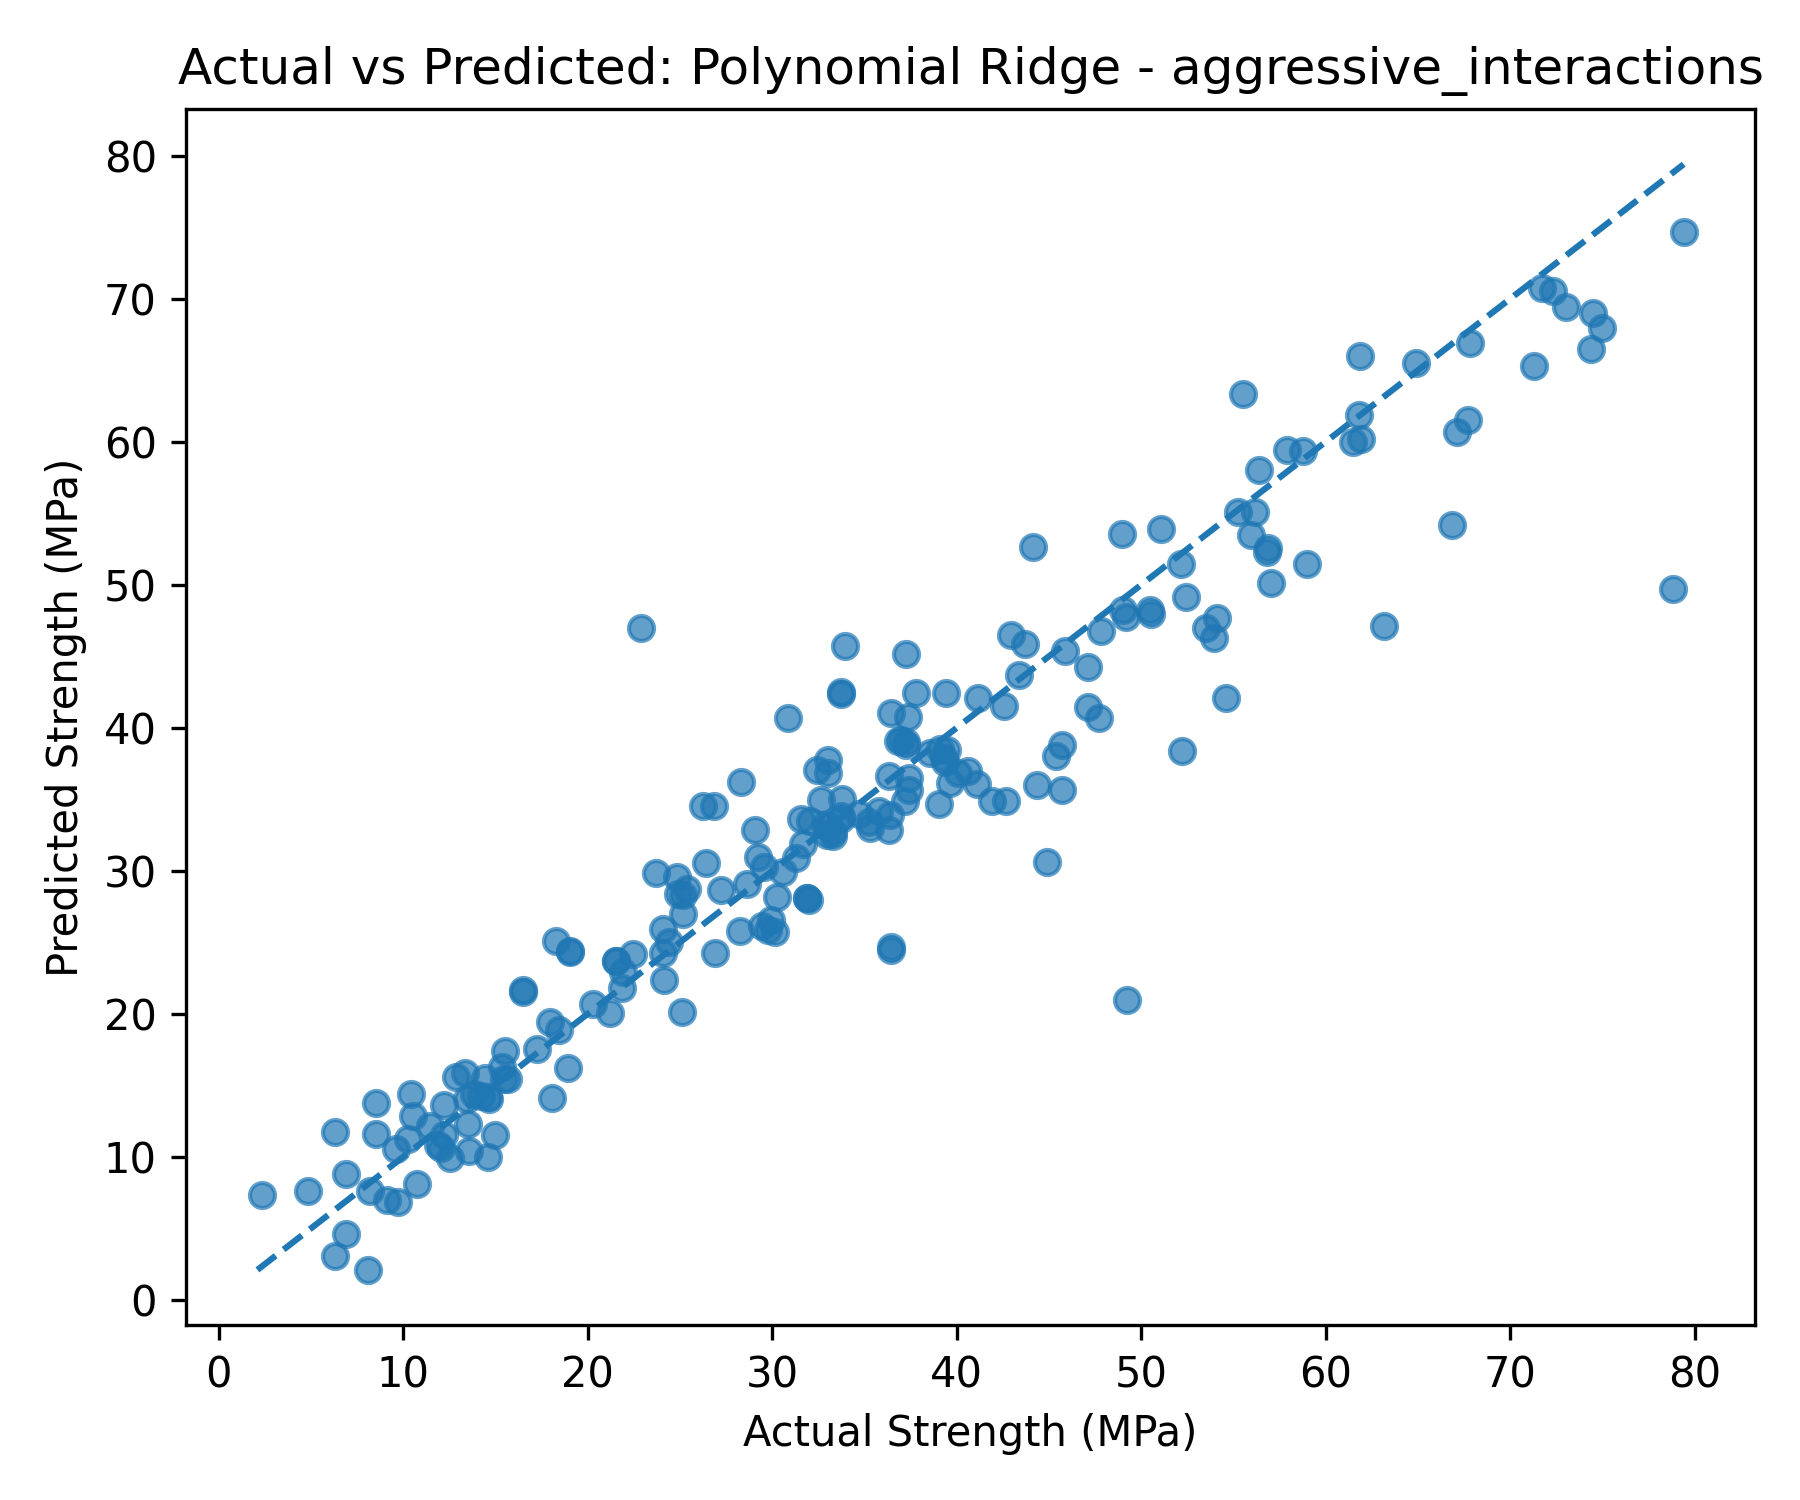
\includegraphics[width=0.48\textwidth]{report_assets/uci_polynomial_actual_vs_predicted.png}
    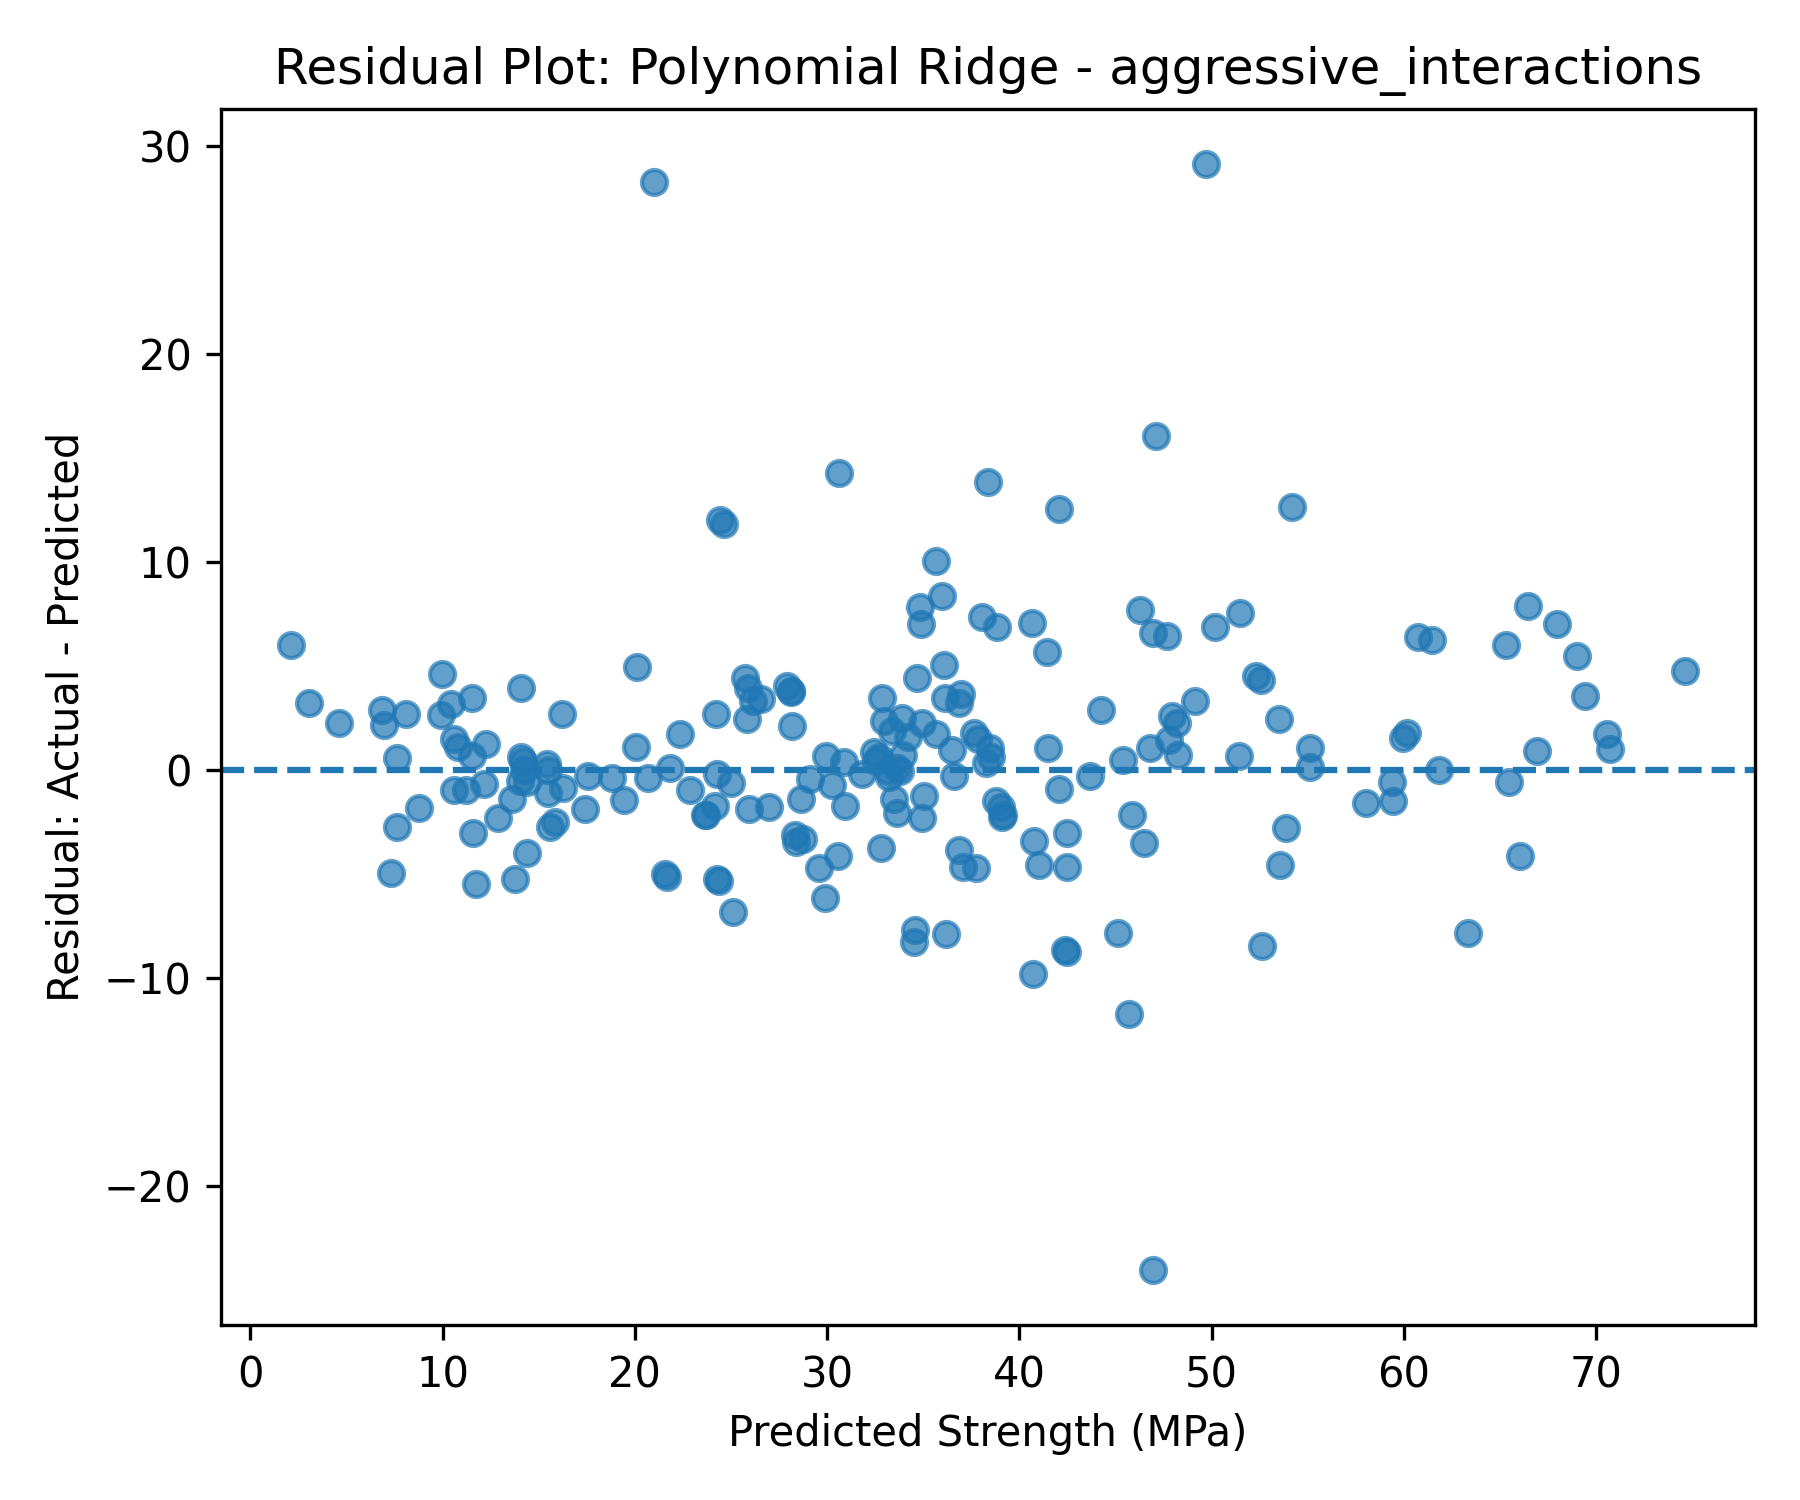
\includegraphics[width=0.48\textwidth]{report_assets/uci_polynomial_residuals.png}
    \caption{UCI Polynomial Ridge predictions and residuals on the held-out test set.}
    \label{fig:uci_poly}
\end{figure}

\subsubsection{UHPC Dataset}

\paragraph{Dataset Variant}
The final UHPC modeling setup used the shared semantic recoding strategy with a 50\% missingness threshold. After keeping rows with valid 28-day compressive strength, 2073 rows remained.

\begin{center}
\begin{tabular}{@{}lrrrr@{}}
\toprule
\textbf{Dataset} & \textbf{Rows} & \textbf{Raw Predictors} & \textbf{Numeric} & \textbf{Categorical} \\
\midrule
Source data with publication metadata & 2073 & 34 & 24 & 9 \\
Modeling data without publication     & 2073 & 33 & 24 & 9 \\
Encoded model matrix                  & 2073 & 60 & -- & -- \\
\bottomrule
\end{tabular}
\end{center}

\paragraph{Final Model Performance (Random Split)}
The row-mixed split used 1449 training rows, 311 validation rows, and 313 test rows. Identical feature vectors were kept in the same split to reduce direct duplicate leakage.

\begin{center}
\begin{tabular}{@{}ll@{}}
\toprule
\textbf{Model} & \textbf{Hyperparameters} \\
\midrule
OLS              & \texttt{\{\}} \\
Elastic Net      & \texttt{alpha=0.01, l1\_ratio=0.3} \\
Bayesian Ridge   & \texttt{alpha\_1=1e-05, lambda\_1=1e-07} \\
Polynomial Ridge & \texttt{degree=2, alpha=100.0} \\
\bottomrule
\end{tabular}
\end{center}

\vspace{0.3cm}

\begin{center}
\begin{tabular}{@{}lrrrrrrr@{}}
\toprule
\textbf{Model} & \textbf{CV RMSE} & \multicolumn{3}{c}{\textbf{Validation}} & \multicolumn{3}{c}{\textbf{Test}} \\
 & & \textbf{RMSE} & \textbf{MAE} & \textbf{$R^2$} & \textbf{RMSE} & \textbf{MAE} & \textbf{$R^2$} \\
\midrule
OLS              & --    & 21.96 & 16.97 & 0.662 & 21.09 & 16.56 & 0.685 \\
Elastic Net      & 23.97 & 21.75 & 16.98 & 0.669 & 20.91 & 16.54 & 0.690 \\
Bayesian Ridge   & 24.03 & 21.74 & 16.99 & 0.669 & 20.93 & 16.56 & 0.689 \\
Polynomial Ridge & 19.83 & 343.34 & 30.65 & -81.54 & 15.51 & 11.14 & 0.829 \\
\bottomrule
\end{tabular}
\end{center}

\paragraph{Interpretation}
Elastic Net and Bayesian Ridge were the most reliable UHPC models. Polynomial Ridge had the best test score, but its validation error was extremely unstable, so it was not selected as the main UHPC model. Bayesian Ridge had the lowest stable validation RMSE, while Elastic Net was retained for the publication-held-out and attribution analyses because it was sparse, stable, and easy to interpret.

\begin{figure}[H]
    \centering
    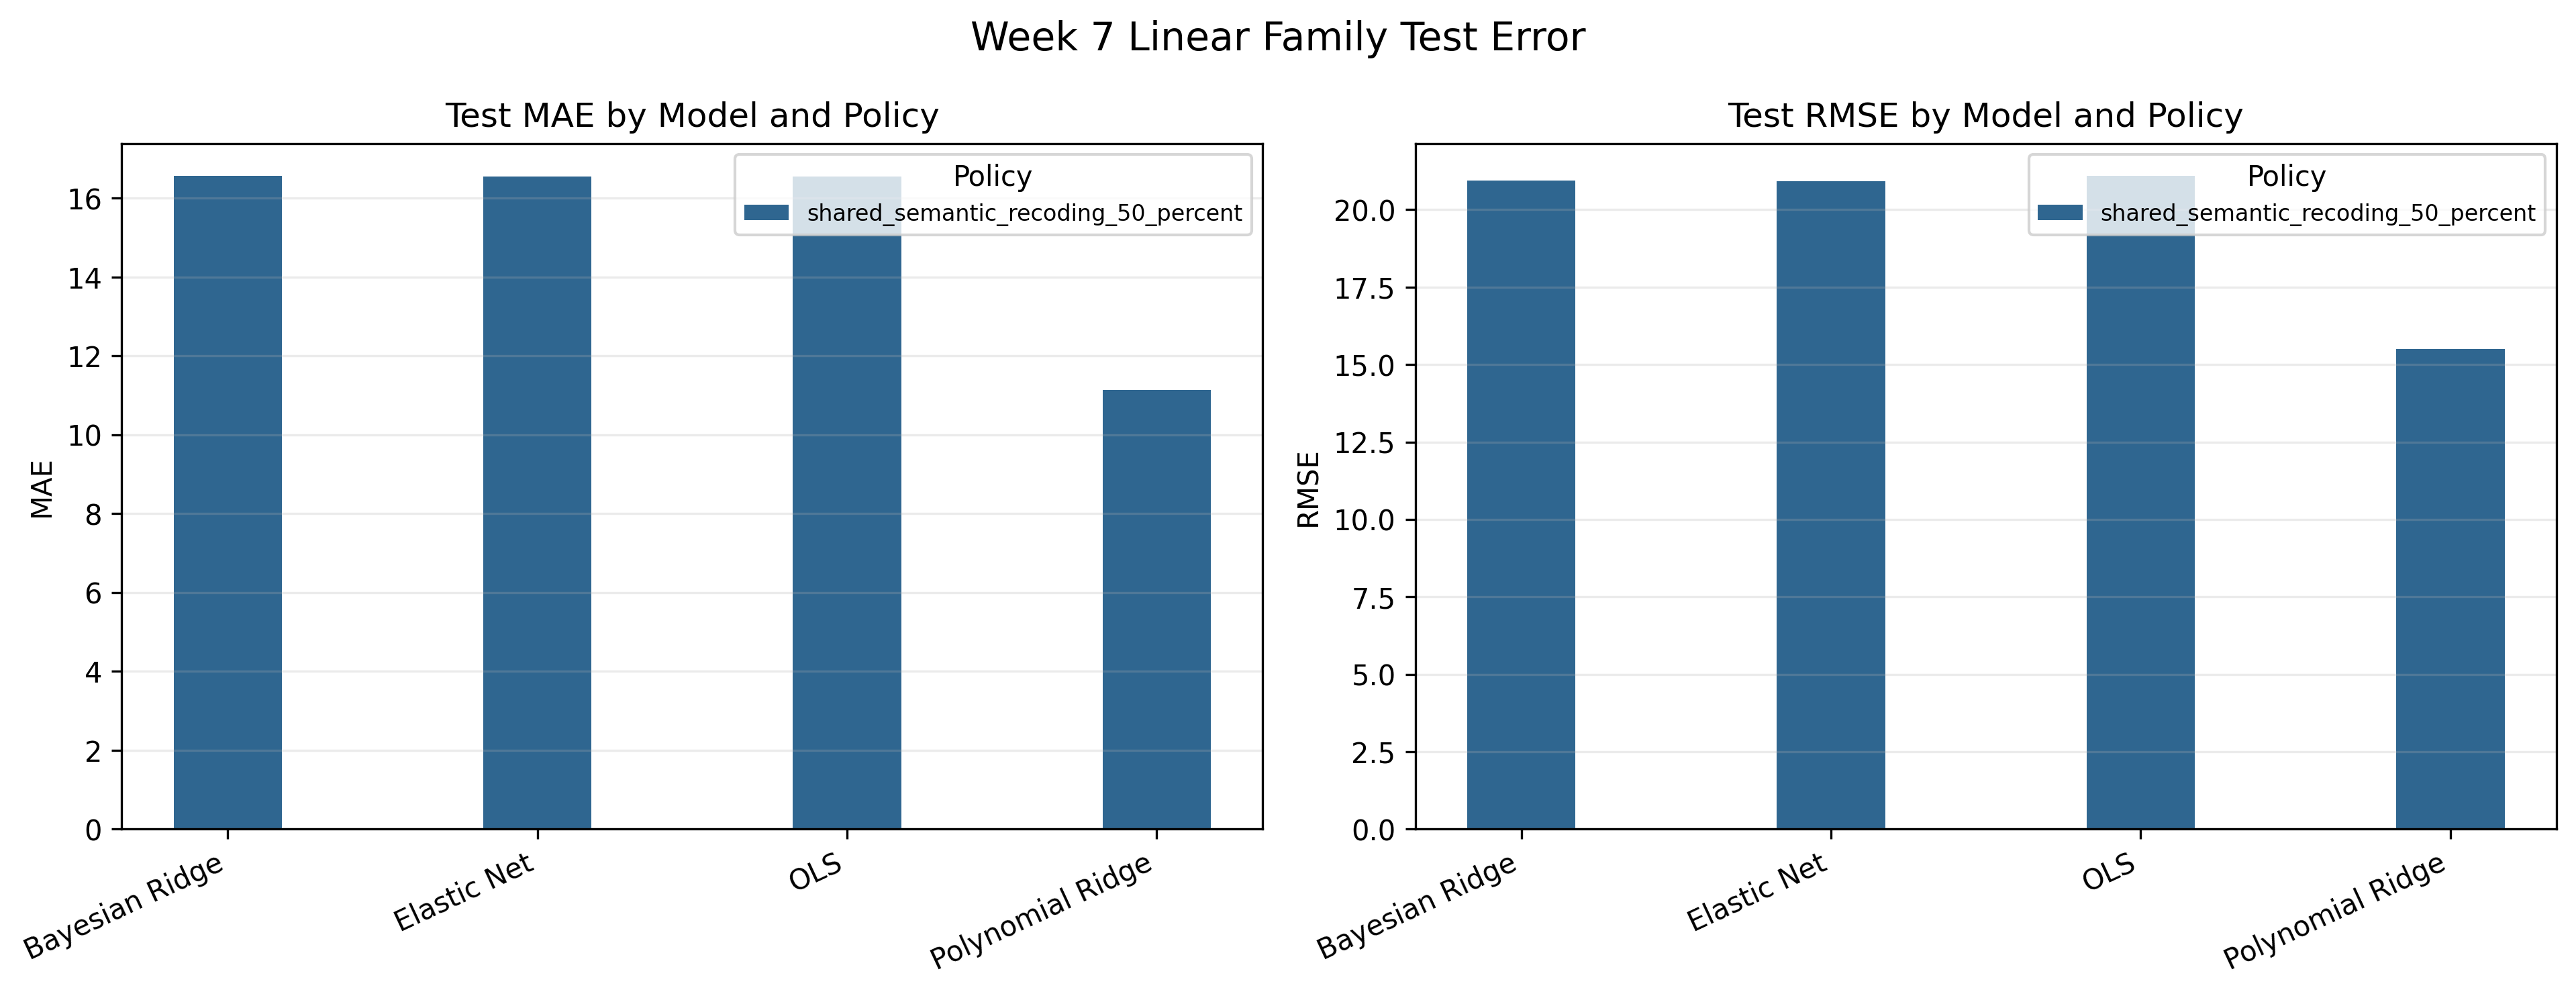
\includegraphics[width=0.88\textwidth]{report_assets/uhpc_row_mixed_metrics.png}
    \caption{Row-mixed UHPC performance for the Linear Model Family.}
    \label{fig:uhpc_row_mixed}
\end{figure}

\clearpage

\subsection{Targeted Experiments}
This subsection checks how sensitive the UHPC linear models are to fibre information, outliers, engineered ratios, and multicollinearity.

\paragraph{Removing All Fibre Columns}
All fibre amount, type, length, and diameter features were removed. This reduced the predictive power of the stable linear models.

\begin{center}
\small
\begin{tabular}{@{}lrrrr@{}}
\toprule
\textbf{Model} & \textbf{Base RMSE} & \textbf{No-Fibre RMSE} & \textbf{Base $R^2$} & \textbf{No-Fibre $R^2$} \\
\midrule
OLS              & 21.09 & 24.08 & 0.685 & 0.589 \\
Elastic Net      & 20.91 & 23.94 & 0.690 & 0.594 \\
Bayesian Ridge   & 20.93 & 23.97 & 0.689 & 0.593 \\
Polynomial Ridge & 15.51 & 20.36 & 0.829 & 0.706 \\
\bottomrule
\end{tabular}
\end{center}

\paragraph{Outlier Sensitivity}
The lower and upper 2.5\% of training targets were removed, reducing the training set from 1449 to 1375 rows. This did not improve generalization.

\begin{center}
\small
\begin{tabular}{@{}lrrrr@{}}
\toprule
\textbf{Model} & \textbf{Base RMSE} & \textbf{No-Outlier RMSE} & \textbf{Base $R^2$} & \textbf{No-Outlier $R^2$} \\
\midrule
OLS              & 21.09 & 22.41 & 0.685 & 0.644 \\
Elastic Net      & 20.91 & 22.35 & 0.690 & 0.646 \\
Bayesian Ridge   & 20.93 & 22.64 & 0.689 & 0.636 \\
Polynomial Ridge & 15.51 & 16.45 & 0.829 & 0.808 \\
\bottomrule
\end{tabular}
\end{center}

\paragraph{Engineered Ratio Features}
Adding domain ratios did not improve the stable models. Elastic Net test RMSE changed from 20.91 to 21.39, and Bayesian Ridge changed from 20.93 to 21.41. This suggests that the existing composition variables already carried most of the useful linear information.

\paragraph{VIF Diagnostic}
The numeric predictors did not show severe multicollinearity. The maximum VIF was 3.81, the median VIF was 1.60, and no feature had VIF above 5.

\subsection{Publication-Level Generalisation}
Random row splits can be optimistic because rows from the same paper may share materials, equipment, and reporting style. Therefore, the UHPC model was also tested by holding out complete publications.

\paragraph{Publication-Held-Out Split}
\begin{center}
\begin{tabular}{@{}lrrrr@{}}
\toprule
\textbf{Split} & \textbf{Rows} & \textbf{Publications} & \textbf{Target Mean} & \textbf{Target Std.} \\
\midrule
Train      & 1451 & 115 & 145.91 & 34.59 \\
Validation & 311  & 25  & 152.21 & 34.95 \\
Test       & 311  & 25  & 168.15 & 40.08 \\
\bottomrule
\end{tabular}
\end{center}

\paragraph{Row-Mixed vs. Publication-Held-Out Test}
\begin{center}
\begin{tabular}{@{}lrrrrr@{}}
\toprule
\textbf{Evaluation} & \textbf{Rows} & \textbf{Model} & \textbf{MAE} & \textbf{RMSE} & \textbf{$R^2$} \\
\midrule
Row-mixed test              & 313 & Elastic Net & 16.73 & 21.21 & 0.681 \\
Publication-held-out test   & 311 & Elastic Net & 25.79 & 30.22 & 0.430 \\
\bottomrule
\end{tabular}
\end{center}

\paragraph{LOPO Summary}
\begin{center}
\begin{tabular}{@{}lrrrrr@{}}
\toprule
\textbf{Aggregation} & \textbf{Publications} & \textbf{Rows} & \textbf{MAE} & \textbf{RMSE} & \textbf{$R^2$} \\
\midrule
Micro average over rows        & 6 & 452 & 24.82 & 29.74 & 0.160 \\
Equal publication average      & 6 & 452 & 24.75 & 29.61 & -1.045 \\
\bottomrule
\end{tabular}
\end{center}

\paragraph{Interpretation}
The publication-held-out result is much weaker than the row-mixed result. RMSE increased by about 9 MPa and $R^2$ dropped from 0.681 to 0.430. This shows that the linear model transfers less well to unseen publications than the row-mixed score first suggests.

\begin{figure}[H]
    \centering
    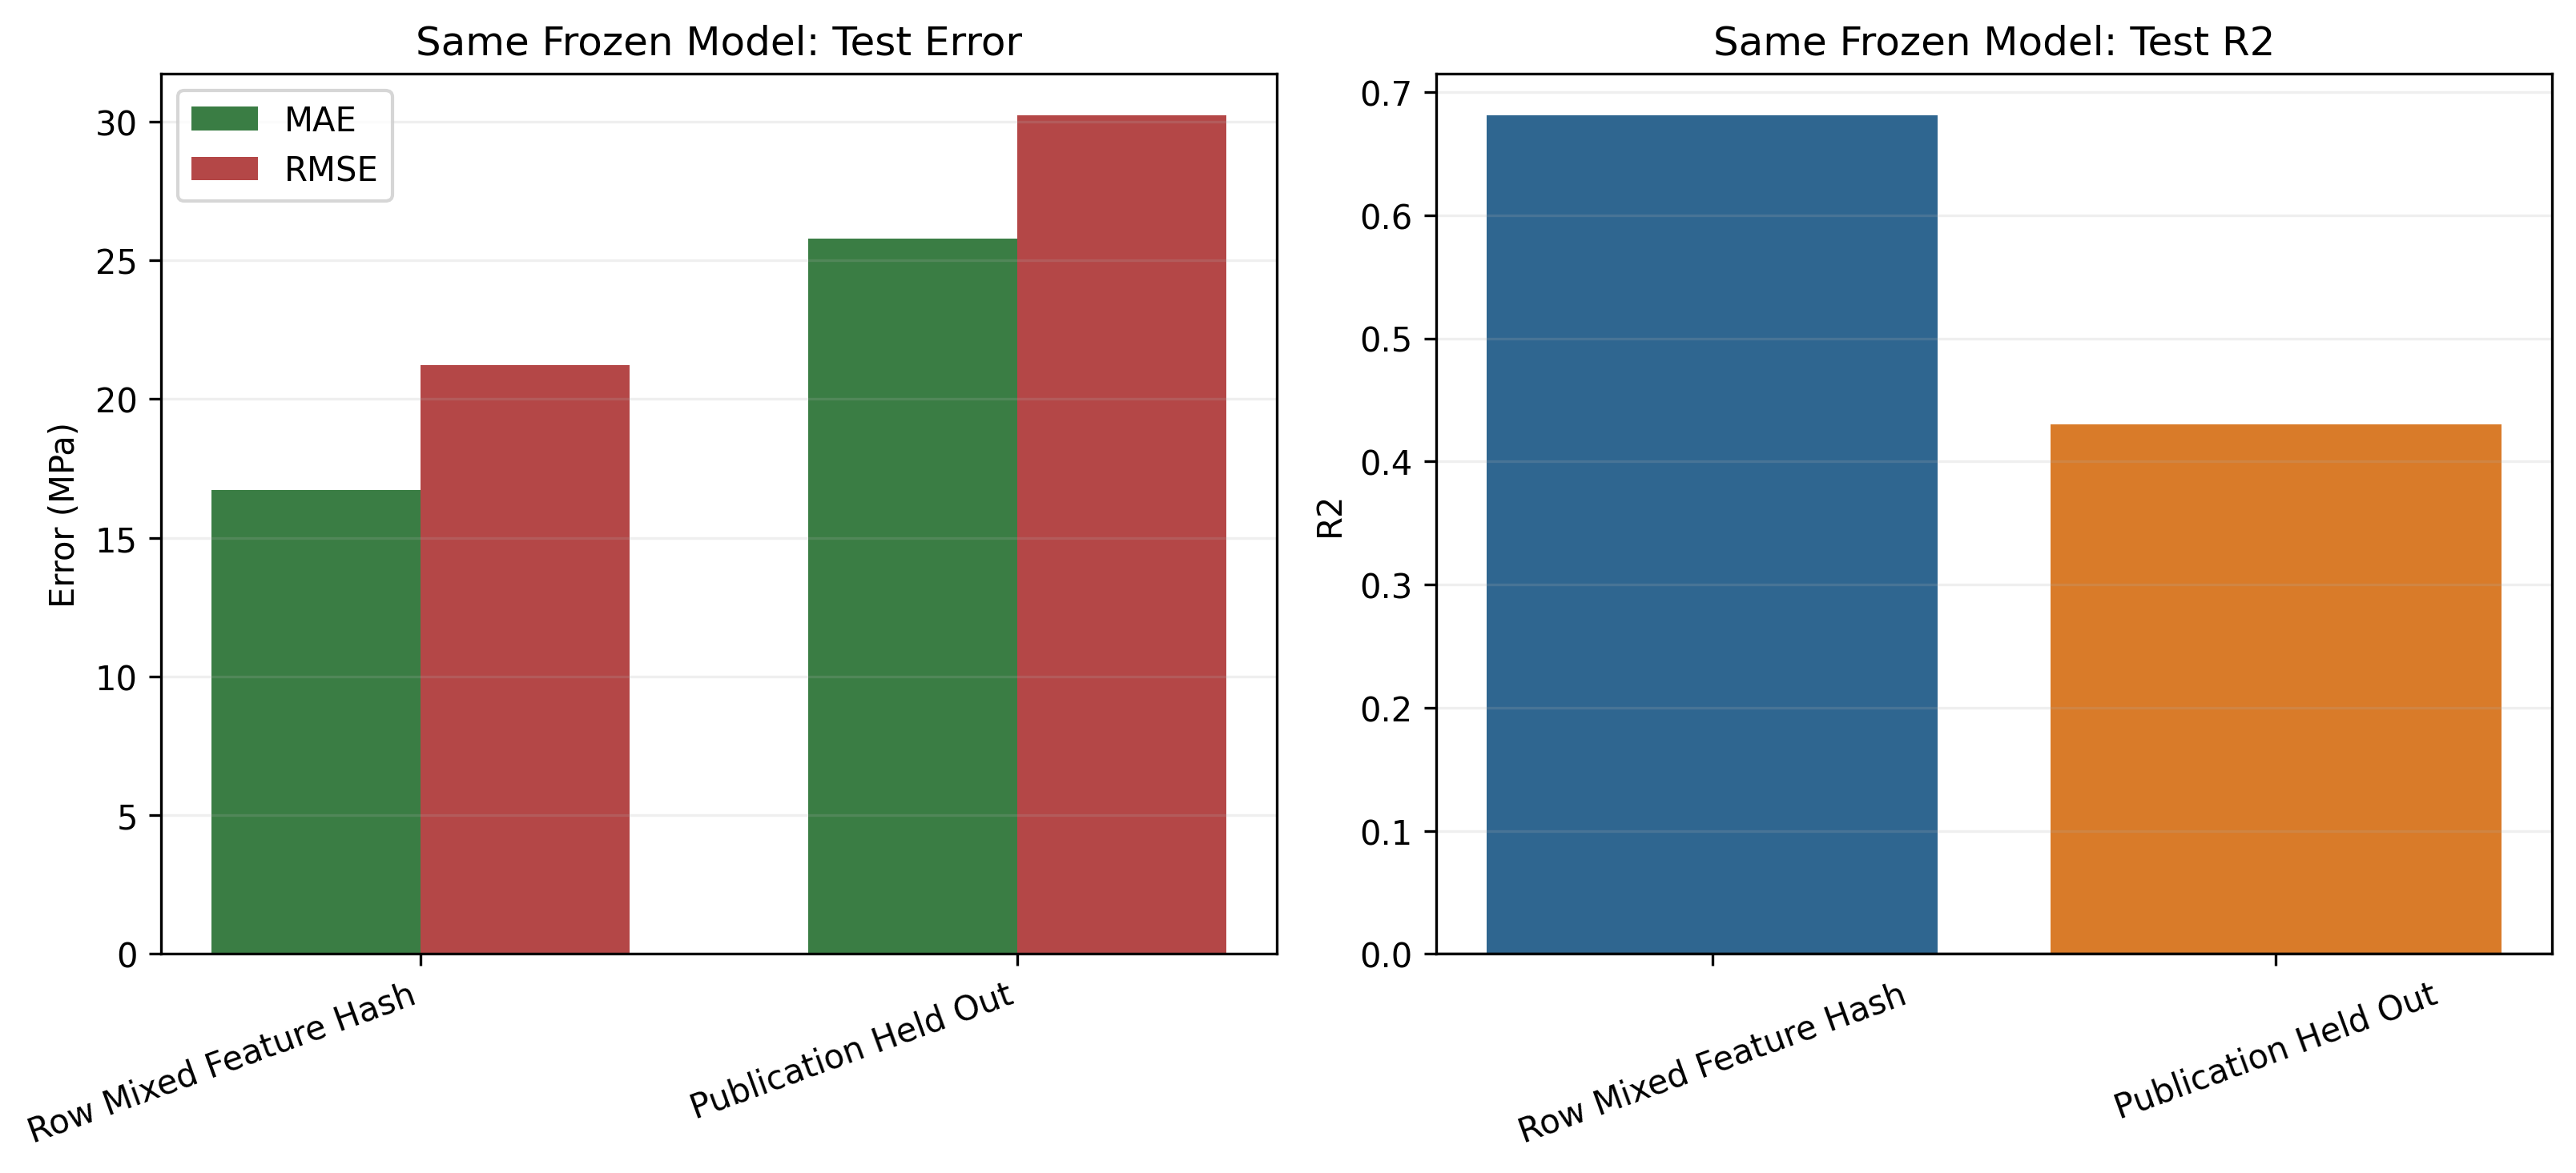
\includegraphics[width=0.78\textwidth]{report_assets/publication_generalization_gap.png}
    \caption{Generalisation gap between row-mixed and publication-held-out testing.}
    \label{fig:publication_gap}
\end{figure}

\clearpage

\subsection{Uncertainty and Calibration}
Prediction intervals were evaluated at the 90\% nominal coverage level on the publication-held-out test set.

\begin{center}
\begin{tabular}{@{}llrrrr@{}}
\toprule
\textbf{Method} & \textbf{Model} & \textbf{Coverage} & \textbf{Width} & \textbf{RMSE} & \textbf{$R^2$} \\
\midrule
Split conformal              & Elastic Net    & 0.894 &  94.46 & 28.49 & 0.493 \\
Native interval              & Bayesian Ridge & 0.830 &  85.11 & 27.72 & 0.520 \\
Conformalized interval       & Bayesian Ridge & 0.936 & 108.02 & 27.72 & 0.520 \\
Residual bootstrap           & Elastic Net    & 0.743 &  66.94 & 28.49 & 0.493 \\
Bootstrap conformalized      & Elastic Net    & 0.916 &  95.15 & 28.49 & 0.493 \\
\bottomrule
\end{tabular}
\end{center}

\paragraph{LOPO Calibration Summary}
\begin{center}
\begin{tabular}{@{}llrrrr@{}}
\toprule
\textbf{Method} & \textbf{Model} & \textbf{Coverage} & \textbf{Width} & \textbf{RMSE} & \textbf{$R^2$} \\
\midrule
Split conformal              & Elastic Net    & 0.938 & 101.90 & 29.46 & 0.176 \\
Native interval              & Bayesian Ridge & 0.754 &  77.80 & 30.31 & 0.128 \\
Conformalized interval       & Bayesian Ridge & 0.931 & 101.29 & 30.31 & 0.128 \\
Residual bootstrap           & Elastic Net    & 0.777 &  70.63 & 29.46 & 0.176 \\
Bootstrap conformalized      & Elastic Net    & 0.925 &  99.57 & 29.46 & 0.176 \\
\bottomrule
\end{tabular}
\end{center}

\paragraph{Interpretation}
The conformal methods were closest to the desired 90\% coverage. However, the intervals were wide, usually around 95--102 MPa. This means that the model can express uncertainty, but predictions for unseen publications should still be treated carefully.

\begin{figure}[H]
    \centering
    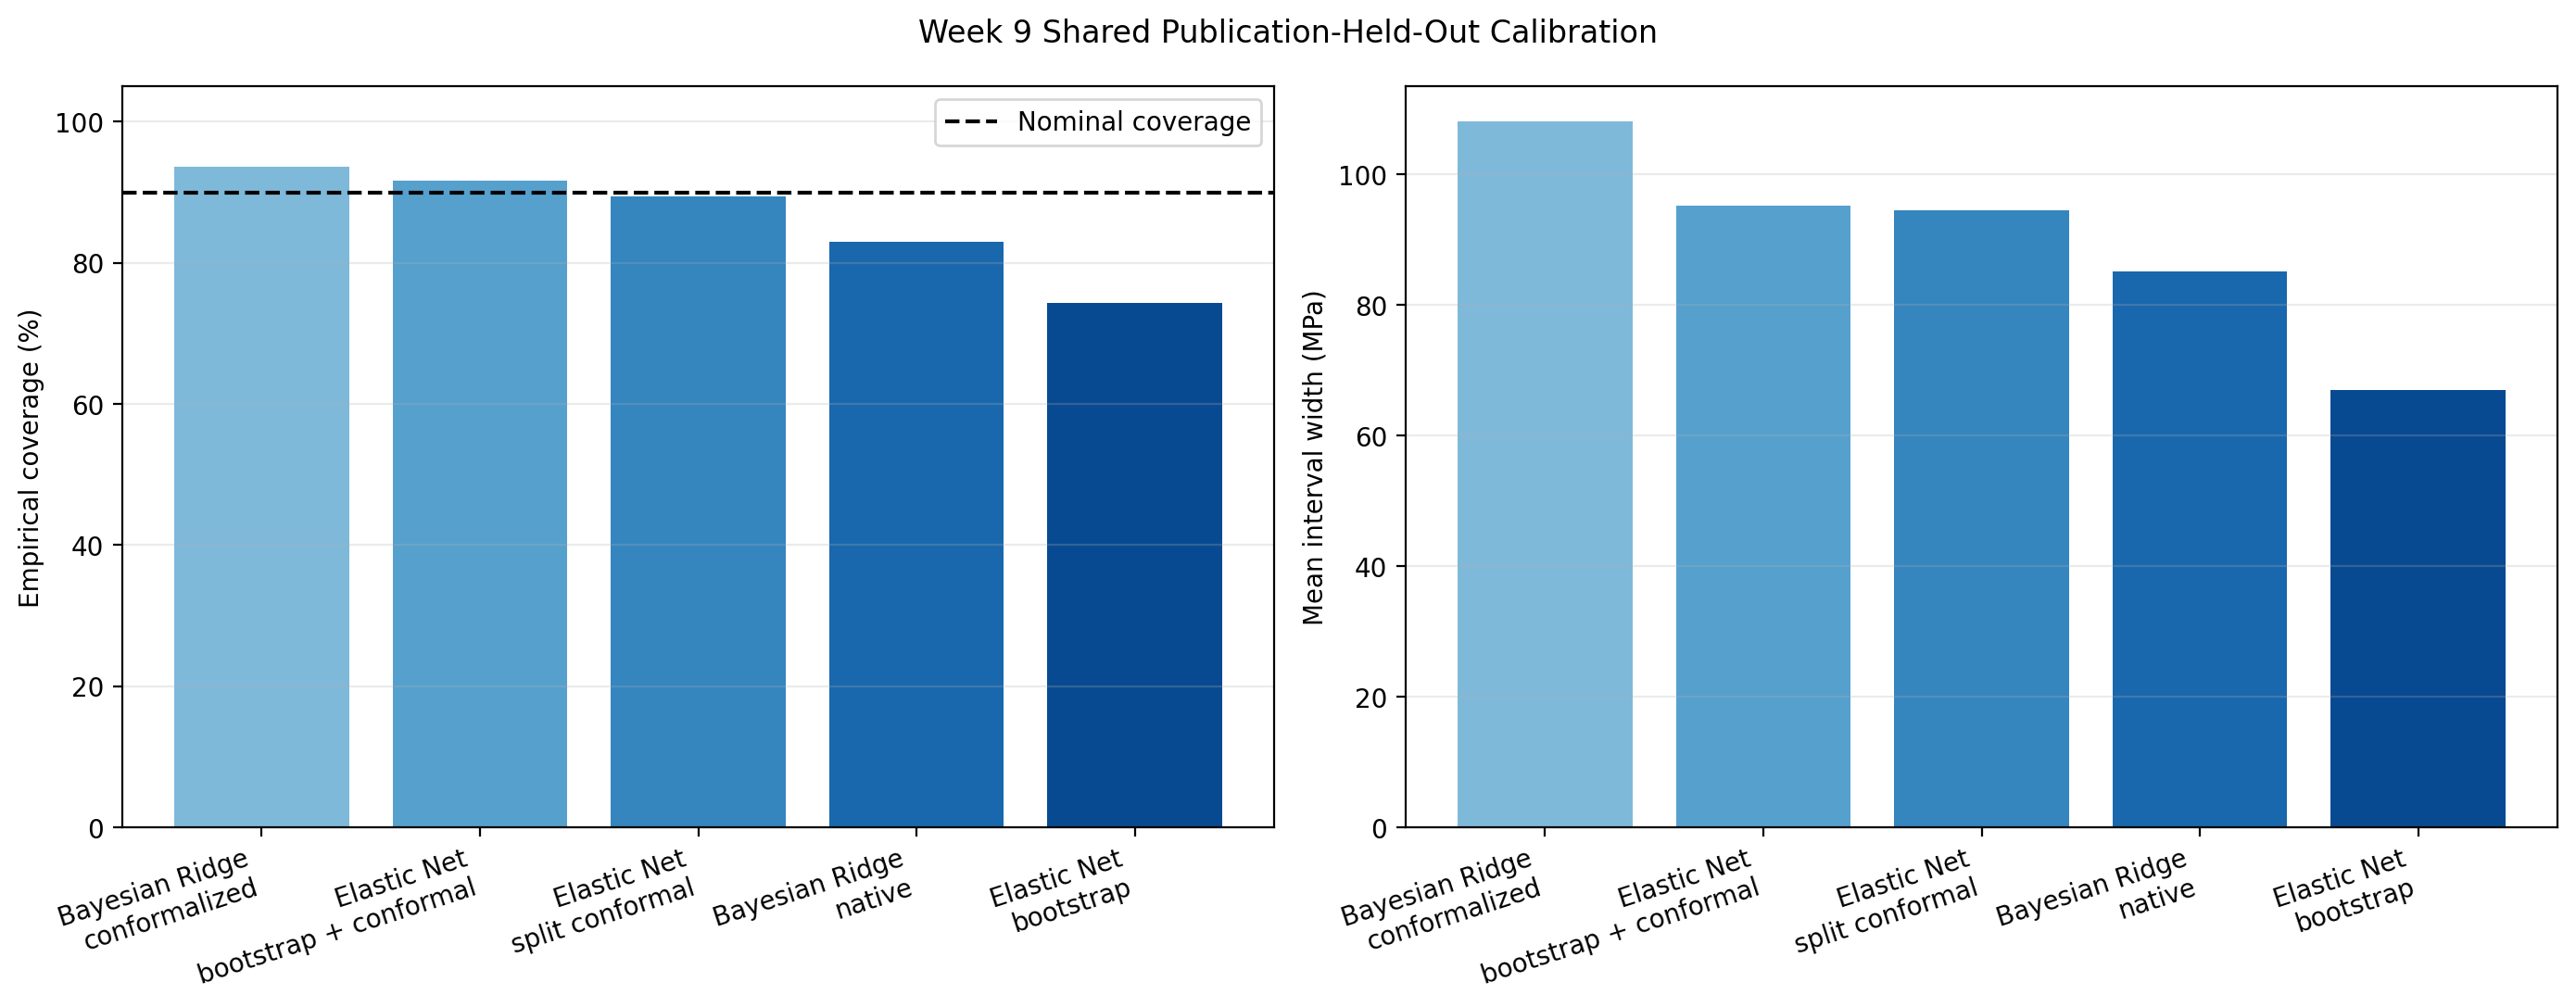
\includegraphics[width=0.78\textwidth]{report_assets/uncertainty_coverage_width.png}
    \caption{Coverage and interval width for the publication-held-out uncertainty methods.}
    \label{fig:uncertainty}
\end{figure}

\subsection{Combined Error, Uncertainty and Explanation Analysis}
This subsection applies to the UHPC dataset only. SHAP and permutation importance were computed for the final Elastic Net model on the publication-held-out test set. Grouped SHAP is reported as the sum of individual feature mean-absolute SHAP values inside each physical group.

\paragraph{Readiness Check}
The attribution audit passed: the test rows, targets, and lineage rows were aligned (311/311/311), publication metadata was not present in the predictors, SHAP additivity error was $2.84 \times 10^{-14}$, and permutation importance reused the fitted model without refitting.

\paragraph{Elastic Net: Grouped Feature Attribution vs. Permutation Importance}
\begin{table}[H]
\centering
\caption{Elastic Net --- Grouped Feature Attribution vs.\ Permutation Importance}
\label{tab:elastic_group_importance}
\begin{tabular}{lrrr}
\toprule
Feature Group & SHAP Mean & Permutation Mean RMSE & Permutation Std \\
\midrule
Binders and SCMs        & 21.4954 & 0.8616 & 0.4303 \\
Curing                  & 13.8516 & 8.5186 & 0.8489 \\
Fillers and Aggregates  & 11.0776 & 2.2498 & 0.2913 \\
Fibres                  & 10.0854 & 3.8381 & 0.5073 \\
Chemical Admixtures     &  3.8011 & 0.2495 & 0.1789 \\
Water                   &  2.7843 & 0.5347 & 0.1202 \\
\bottomrule
\end{tabular}
\end{table}

\paragraph{Elastic Net: Top 10 Individual Raw Features by SHAP Mean}
\begin{table}[H]
\centering
\caption{Elastic Net --- Top 10 Individual Raw Features by SHAP Mean}
\label{tab:elastic_top10_features}
\begin{tabular}{lrrr}
\toprule
Feature & SHAP Mean & Permutation Mean RMSE & Permutation Std \\
\midrule
curing\_temp     & 12.2728 & 8.5350 & 0.8266 \\
sand\_type       &  7.6199 & 1.3389 & 0.3843 \\
fiber1\_amount   &  6.5705 & 2.3305 & 0.4192 \\
fly\_ash\_type    &  5.1856 & 0.5348 & 0.2892 \\
cement\_type     &  3.4299 & 0.4082 & 0.1611 \\
silica\_fume     &  3.3745 & 1.0121 & 0.1847 \\
fly\_ash         &  3.1480 & 0.5071 & 0.1311 \\
fiber1\_type     &  2.9135 & 0.5736 & 0.1390 \\
water            &  2.7843 & 0.5399 & 0.1311 \\
sp\_type         &  2.1885 & 0.8631 & 0.1467 \\
\bottomrule
\end{tabular}
\end{table}

\paragraph{Interpretation}
The SHAP and permutation views answer slightly different questions. SHAP assigns large total contribution to binders and SCMs because this group contains many cementitious variables. Permutation importance shows that curing is the most damaging group to shuffle, and \texttt{curing\_temp} is the strongest individual feature by both SHAP and permutation. Therefore, curing is not a mistake in the implementation; it is genuinely important for the linear model, especially when testing on unseen publications.

\begin{figure}[H]
    \centering
    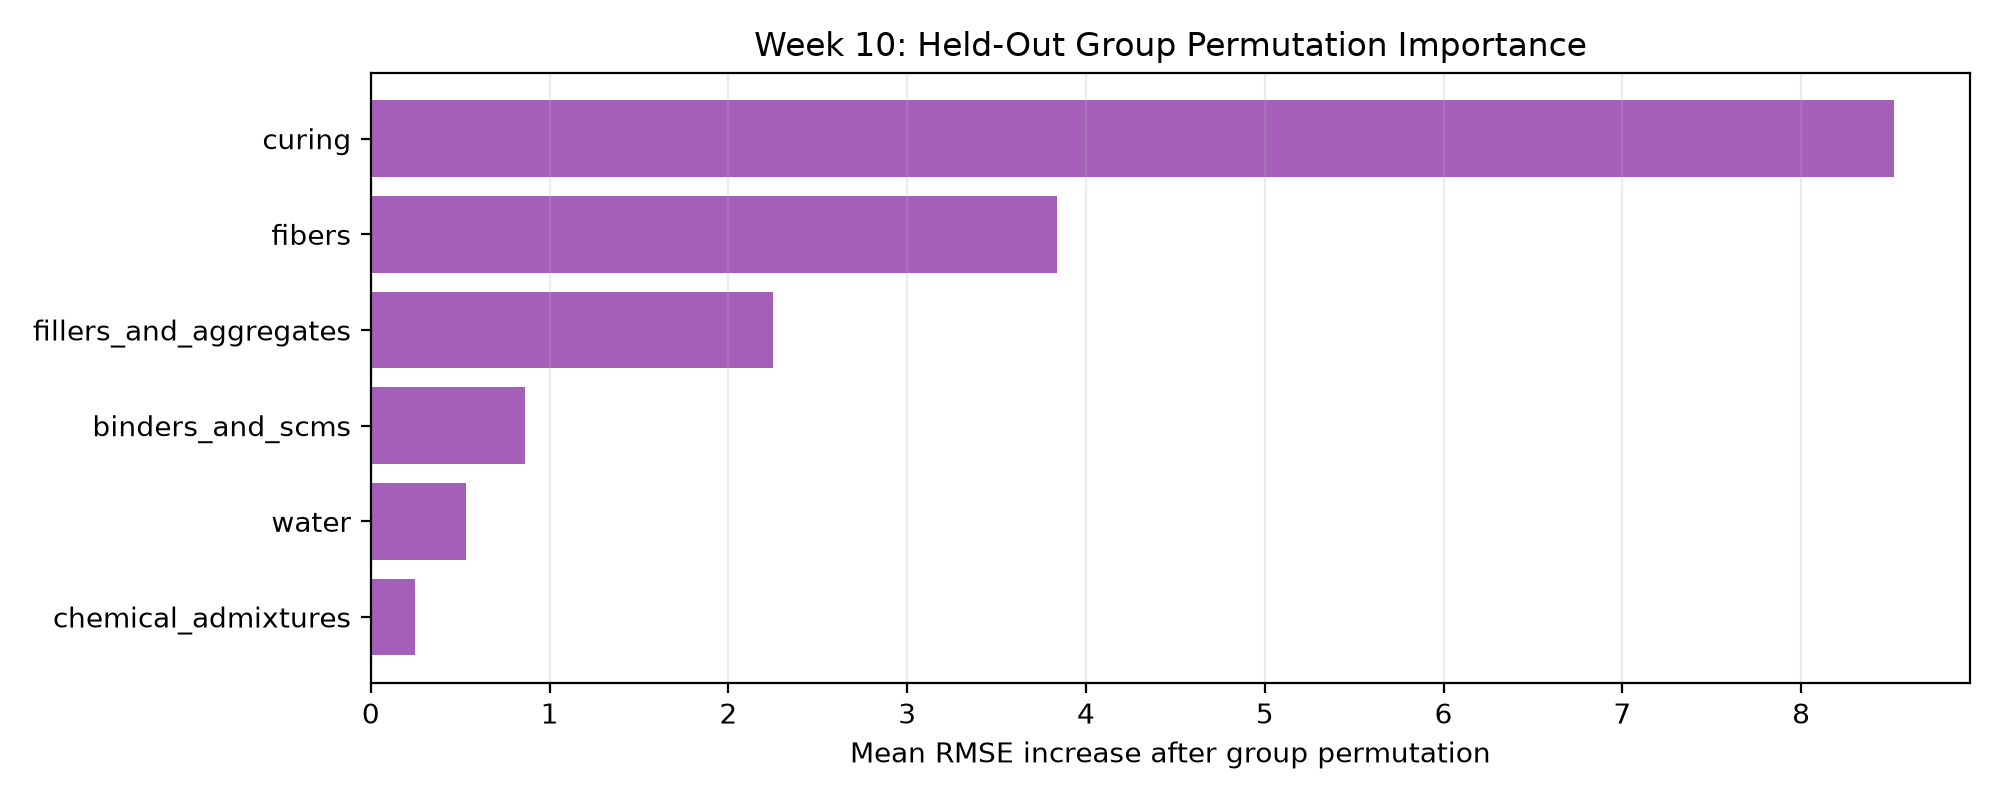
\includegraphics[width=0.72\textwidth]{report_assets/group_permutation_importance.png}
    \caption{Grouped permutation importance for the Elastic Net model on held-out publications.}
    \label{fig:group_permutation}
\end{figure}

\section{Conclusion}
Polynomial Ridge worked very well on the cleaner UCI benchmark, especially after interaction features were added. On UHPC, the stable linear models were less accurate but easier to interpret. The most important finding is the generalisation gap: row-mixed testing looked acceptable, but publication-held-out and LOPO testing showed that unseen publications are much harder. The final explanations are still physically sensible, with curing, fibres, binders, SCMs, fillers, and aggregates all contributing to model behavior.

\begin{thebibliography}{9}
\bibitem{uci}
I.-C. Yeh, Concrete Compressive Strength Dataset, UCI Machine Learning Repository, 2007.

\bibitem{yeh1998}
I.-C. Yeh, ``Modeling of strength of high-performance concrete using artificial neural networks,'' \textit{Cement and Concrete Research}, vol. 28, no. 12, pp. 1797--1808, 1998.
\end{thebibliography}

\end{document}
